\documentclass[bachelor, och, coursework]{SCWorks}
% параметр - тип обучения - одно из значений:
%    spec     - специальность
%    bachelor - бакалавриат (по умолчанию)
%    master   - магистратура
% параметр - форма обучения - одно из значений:
%    och   - очное (по умолчанию)
%    zaoch - заочное
% параметр - тип работы - одно из значений:
%    referat    - реферат
%    coursework - курсовая работа (по умолчанию)
%    diploma    - дипломная работа
%    pract      - отчет по практике
% параметр - включение шрифта
%    times    - включение шрифта Times New Roman (если установлен)
%               по умолчанию выключен
\usepackage{subfigure}
\usepackage{tikz,pgfplots}
\pgfplotsset{compat=1.5}
\usepackage{float}

%\usepackage{titlesec}
\setcounter{secnumdepth}{4}
%\titleformat{\paragraph}
%{\normalfont\normalsize}{\theparagraph}{1em}{}
%\titlespacing*{\paragraph}
%{35.5pt}{3.25ex plus 1ex minus .2ex}{1.5ex plus .2ex}

\titleformat{\paragraph}[block]
{\hspace{1.25cm}\normalfont}
{\theparagraph}{1ex}{}
\titlespacing{\paragraph}
{0cm}{2ex plus 1ex minus .2ex}{.4ex plus.2ex}

% --------------------------------------------------------------------------%


\usepackage[T2A]{fontenc}
\usepackage[utf8]{inputenc}
\usepackage{graphicx}
\graphicspath{ {./images/} }
\usepackage{tempora}

\usepackage[sort,compress]{cite}
\usepackage{amsmath}
\usepackage{amssymb}
\usepackage{amsthm}
\usepackage{fancyvrb}
\usepackage{listings}
\usepackage{listingsutf8}
\usepackage{longtable}
\usepackage{array}
\usepackage[english,russian]{babel}

% \usepackage[colorlinks=true]{hyperref}
\usepackage{url}

\usepackage{underscore}
\usepackage{setspace}
\usepackage{indentfirst} 
\usepackage{mathtools}
\usepackage{amsfonts}
\usepackage{enumitem}
\usepackage{tikz}
% \usepackage{minted}

\newcommand{\eqdef}{\stackrel {\rm def}{=}}
\newcommand{\specialcell}[2][c]{%
\begin{tabular}[#1]{@{}c@{}}#2\end{tabular}}

\renewcommand\theFancyVerbLine{\small\arabic{FancyVerbLine}}

\newtheorem{lem}{Лемма}

\begin{document}

% Кафедра (в родительном падеже)
\chair{теоретических основ компьютерной безопасности и криптографии}

% Тема работы
\title{Разработка программы для выявления RDP-сессий с использованием нейронных сетей}

% Курс
\course{6}

% Группа
\group{631}

% Факультет (в родительном падеже) (по умолчанию "факультета КНиИТ")
\department{факультета КНиИТ}

% Специальность/направление код - наименование
%\napravlenie{09.03.04 "--- Программная инженерия}
%\napravlenie{010500 "--- Математическое обеспечение и администрирование информационных систем}
%\napravlenie{230100 "--- Информатика и вычислительная техника}
%\napravlenie{231000 "--- Программная инженерия}
\napravlenie{10.05.01 "--- Компьютерная безопасность}

% Для студентки. Для работы студента следующая команда не нужна.
% \studenttitle{Студентки}

% Фамилия, имя, отчество в родительном падеже
\author{Токарева Никиты Сергеевича}

% Заведующий кафедрой
\chtitle{} % степень, звание
\chname{Абросимов М. Б.}

%Научный руководитель (для реферата преподаватель проверяющий работу)
\satitle{доцент} %должность, степень, звание
\saname{Гортинский А. В.}

% Руководитель практики от организации (только для практики,
% для остальных типов работ не используется)
% \patitle{к.ф.-м.н.}
% \paname{С.~В.~Миронов}

% Семестр (только для практики, для остальных
% типов работ не используется)
%\term{8}

% Наименование практики (только для практики, для остальных
% типов работ не используется)
%\practtype{преддипломная}

% Продолжительность практики (количество недель) (только для практики,
% для остальных типов работ не используется)
%\duration{4}

% Даты начала и окончания практики (только для практики, для остальных
% типов работ не используется)
%\practStart{30.04.2019}
%\practFinish{27.05.2019}

% Год выполнения отчета
\date{2023}

\maketitle

% Включение нумерации рисунков, формул и таблиц по разделам
% (по умолчанию - нумерация сквозная)
% (допускается оба вида нумерации)
% \secNumbering

%-------------------------------------------------------------------------------------------

\tableofcontents

\intro
В условиях современной цифровой экономики удалённый доступ к информационным системам играет важную роль в обеспечении удобства, 
гибкости и эффективности работы. Одним из наиболее популярных протоколов для удалённого управления компьютерами является Remote 
Desktop Protocol (RDP). Этот протокол широко используется в корпоративных и частных сетях для предоставления безопасного доступа 
к рабочим станциям, серверам и другим устройствам.


Однако вместе с удобством использования RDP остаётся объектом пристального внимания со стороны злоумышленников. Уязвимости протокола 
часто используются для реализации атак, включая подбор паролей методом перебора (brute force), использование слабых паролей, кражу 
данных и распространение вредоносного ПО. В таких условиях задача мониторинга и выявления RDP-трафика в общем потоке сетевых данных 
приобретает особую актуальность.


Основной целью данной работы является разработка программы для автоматического выявления RDP-сессий в сетевом трафике с использованием 
нейронных сетей, а именно модели LSTM (Long Short-Term Memory). Эта модель, благодаря своей способности обрабатывать последовательности данных, 
предоставляет мощный инструмент для анализа характеристик сетевого трафика и классификации его по типу.

Для достижения цели были поставлены следующие задачи:

\begin{itemize}
  \item изучение особенностей протокола RDP и его признаков в сетевом трафике;
  \item разработка метрик для анализа и классификации RDP-трафика;
  \item использование модели LSTM для решения задачи классификации;
  \item реализация программного продукта, способного анализировать сетевой трафик в режиме реального времени и выявлять RDP-сессии;
  \item тестирование программы и оценка её эффективности.
\end{itemize}

Результаты данной работы могут быть полезны для специалистов в области информационной безопасности, системных администраторов, а также 
разработчиков инструментов мониторинга и анализа сетевого трафика.

% \begin{figure}[H]
%   \centering
%   \includegraphics[width=0.9\textwidth]{pics/http2.jpg}
%   \caption{}
%   \label{}
% \end{figure}
\section{Протокол RDP: место в сетях и особенности реализации}

Концепция удалённого доступа к вычислительным ресурсам зародилась в стремлении управлять компьютерами и серверами, находящимися на расстоянии. 
Это позволило пользователям быть независимыми от физического местоположения оборудования, обеспечивая гибкость и эффективность в использовании 
вычислительных мощностей.

Протокол удаленного рабочего стола (Remote Desktop Protocol, RDP) был разработан корпорацией Microsoft в конце 1990-х годов как решение для 
удаленного доступа к компьютерам и серверам. Истоки технологии удаленного доступа уходят в 90-е годы XX века, когда компании начали создавать 
протоколы для управления вычислительными системами на расстоянии. Одним из первых таких протоколов был Citrix ICA, который стал основой для 
создания RDP. Microsoft внедрила эту технологию в свои продукты, начиная с Windows NT Terminal Server 4.0, что значительно упростило удалённую работу.

\subsection{Обзор протокола RDP}

Идея создания RDP была основана на стремлении обеспечить пользователям возможность удалённого управления вычислительными ресурсами, независимо от 
их физического расположения. Эта технология стала важной частью корпоративных сетей, позволив администраторам эффективно управлять серверами, а 
пользователям --- работать с удалёнными рабочими столами. Вначале RDP был ориентирован на работу в режиме точка-точка, но со временем получил 
поддержку многоточечных соединений, что сделало его более универсальным инструментом для совместной работы и администрирования \cite{rdp2}.

RDP является расширением семейства протоколов T.120 и базируется на стандарте T.Share. Его ключевые особенности:

\begin{enumerate}
  \item Многоканальная архитектура: RDP поддерживает до 64 000 виртуальных каналов для передачи различных типов данных, таких как:
  
  \begin{itemize}
    \item данные презентации;
    \item управление периферийными устройствами;
    \item лицензирование;
    \item зашифрованные команды клавиатуры и мыши.
    
  \end{itemize}
  
  \item Безопасность: протокол включает механизмы шифрования, обеспечивающие защиту передаваемых данных. Это делает RDP надёжным выбором для корпоративных сетей;
  
  \item Универсальность: RDP изначально был разработан для работы с различными сетевыми топологиями, включая ISDN, POTS и TCP/IP. Современные версии фокусируются на TCP/IP, обеспечивая широкую совместимость;
  
  \item Оптимизация сетевого трафика: протокол использует компрессию данных и механизмы кадрирования для минимизации сетевых задержек;
  
  \item Поддержка мультимедиа: современные версии RDP включают функции передачи аудио, видео и взаимодействия с периферийными устройствами, такими как принтеры и USB-устройства.
\end{enumerate}


\subsection{Место RDP в стеке протоколов}

Стек протоколов представляет собой набор взаимосвязанных стандартов и правил, определяющих взаимодействие между различными уровнями сетевой 
архитектуры. Каждый уровень отвечает за выполнение определённых функций, начиная от передачи данных через физические среды до обеспечения 
высокого уровня абстракции для приложений. Существует несколько моделей сетевых взаимодействий, каждая из которых предлагает свой подход 
к организации передачи данных между устройствами в сети.

Наиболее известным примером стека протоколов является модель OSI (Open Systems Interconnection), которая состоит из семи уровней:

\begin{enumerate}
  \item Физический уровень, который отвечает за передачу последовательности битов через канал связи.
  \item Канальный уровень, где осуществляется разбиение данных на <<кадры>>, размер которых обычно достигает
  от несколько сотен до нескольких тысяч байтов.
  \item Сетевой уровень, на котором осуществляется структуризация и маршрутизация пакетов от отправителя к получателю.
  \item Транспортный уровень, функцией которого является передача надежных последовательностей данных произвольной
  длины через коммуникационную сеть от отправителя к получателю.
  \item Сеансовый уровень, на котором происходит поддержка сессии связи, уп-\\*равление взаимодействием между приложениями.  
  \item Уровень представления, который представляет данные в понятном для какой-либо конкретной машины виде.
  \item Прикладной уровень, предоставляющий набор интерфейсов для взаимодействия пользовательских процессов с сетью \cite{osi-model}.
\end{enumerate}

Вследствие этого, RDP является непосредственно протоколом прикладного уровня модели OSI, наряду с HTTP, FTP, SSH и многими другими. Стоит отметить, что 
в основном OSI применяется преимущественно в образовательных и теоретических целях. На практике используется модель TCP/IP, которая отражает
реальную организацию современных компьютерных сетей \cite{stack}. Она была разработана как часть стека протоколов, лежащих в основе интернета. 
Название TCP/IP связано с двумя ключевыми протоколами этого семейства — Transmission Control Protocol (TCP) и Internet Protocol (IP). Именно они 
были впервые разработаны и задокументированы в этом стандарте. Иногда эту модель называют моделью DOD (Department of Defense).
TCP/IP используется повсеместно, поскольку большинство современных протоколов (HTTP, FTP, RDP) работают в рамках этой модели. Модель TCP/IP 
разделяет сетевое взаимодействие на четыре уровня, каждый из которых выполняет определённые функции:

\begin{enumerate}
    \item Сетевой интерфейс/канальный уровень (объединяет уровни 1 и 2 OSI): отвечает за физическую передачу данных.
    \item Сетевой уровень (аналог уровня 3 OSI): используется для маршрутизации данных (например, протокол IP).
    \item Транспортный уровень (аналог уровня 4 OSI): обеспечивает надежность передачи данных с помощью протоколов TCP и UDP.
    \item Прикладной уровень (соответствует уровням 5, 6 и 7 OSI): поддерживает приложения и службы, такие как HTTP, FTP, RDP и т.д.
\end{enumerate}

Основное преимущество TCP/IP в том, что это практическая модель, на основе которой построен интернет. Все современные сети работают 
с протоколами TCP/IP, поэтому в реальных системах она имеет приоритет.

Здесь важно понимать, что в компьтерных сетях все данные инкапсулируются и декапсулируются на различных уровнях модели TCP/IP.
Процесс инкапсуляции происходит так, что на каждом уровне стека 
протоколы добавляют свои заголовки: от уровня приложений до канального уровня. На этапе приема данные декапсулируются в обратном порядке, начиная 
с канального уровня и заканчивая уровнем приложений. 

Исходя из описания уровней, RDP в модели TCP/IP также относится к прикладному уровню. Поэтому, данные RDP сначала инкапсулируются в сегменты TCP, 
которые затем оборачиваются в IP-пакеты и кадры Ethernet для передачи по сети. На принимающем устройстве данные декапсулируются в обратном 
порядке, начиная с канального уровня и заканчивая уровнем приложений, уровнем RDP.

Для понимания процесса передачи данных от отправителя к получателю важно рассмотреть структуру пакетов, используемых в сетевых взаимодействиях. Далее
будет рассмотрена четырехуровневая структура модели TCP/IP от канального до прикладного. 


\subsubsection{Структура Ethernet-кадра}

На канальном уровне передача данных осуществляется с использованием Ethernet-кадра. Его структура представлена на рисунке \ref{eth-frame}.

\begin{figure}[H]
  \centering
  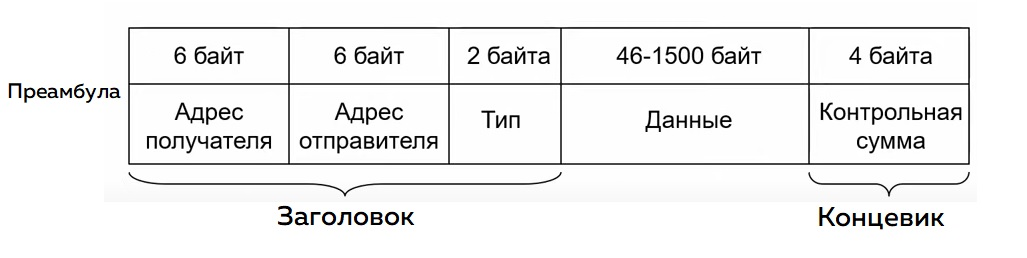
\includegraphics[width=0.9\textwidth]{pics/eth-frame.jpg}
  \caption{Структура Ethernet кадра}
  \label{eth-frame}
\end{figure}

Ключевыми полями Ethernet-кадра являются:

\begin{itemize}
  \item MAC-адреса источника и назначения --- позволяют определить отправителя и получателя на канальном уровне.
  \item Поле <<Тип>> --- указывает номер инкапсулированного сетевого протокола (например, IPv4 или IPv6).
  \item Поле данных --- содержит инкапсулированные данные более высокого уровня, включая сетевые пакеты.
\end{itemize}

\subsubsection{Структура IPv4-заголовка}

Для передачи TCP-сегментов на сетевом уровне используется IP-протокол. В данной работе рассматривается версия IPv4, 
так как её возможностей достаточно для анализа RDP-трафика. Структура IPv4-заголовка представлена на рисунке \ref{ipv4-header}.

\begin{figure}[H]
  \centering
  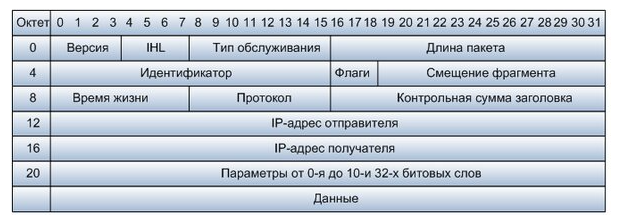
\includegraphics[width=0.9\textwidth]{pics/ipv4-header.png}
  \caption{Структура IPv4-заголовка}
  \label{ipv4-header}
\end{figure}

Особо важны следующие поля IPv4-заголовка:

\begin{itemize}
  \item IP-адреса отправителя и получателя --- позволяют идентифицировать ус-\\*тройства, участвующие в обмене данными.
  \item Поле <<Протокол>> --- определяет протокол транспортного уровня. Например, значение 6 указывает на TCP, а 17 --- на UDP.
\end{itemize}

\subsubsection{Структура заголовков TCP и UDP}

Известно, что протокол RDP взаимодействует с транспортным уровнем через TCP и UDP.
В основном данный протокол использует TCP для установления надёжного соединения и передачи данных, что позволяет обеспечить стабильное взаимодействие 
между клиентом и сервером удалённого рабочего стола. Сама структура TCP-заголовка показана на рисунке \ref{tcp-header}.

  \begin{figure}[H]
    \centering
    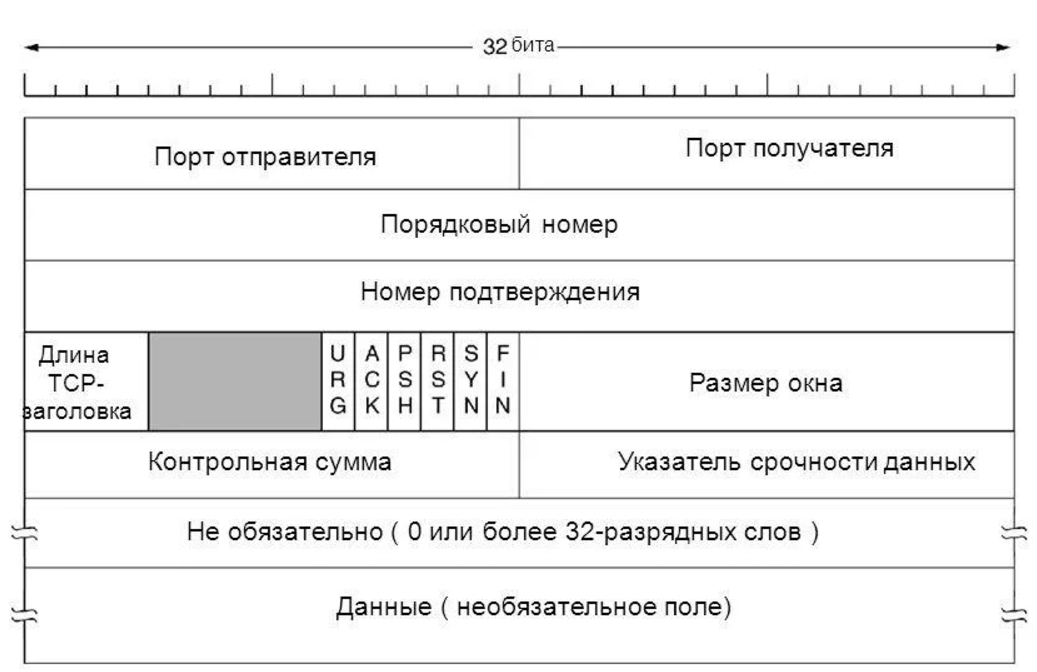
\includegraphics[width=0.9\textwidth]{pics/tcp-segment.png}
    \caption{Структура TCP-заголовка}
    \label{tcp-header}
  \end{figure}

В данном сегменте одними из интересных полей является информация о портах отправителя и получателя. Стоит отметить, что при подключении к 
удаленному рабочему столу по умолчанию используется порт 3389, что помогает идентифицировать RDP-трафик.

Не менее интересным полей является поле <<Размер окна>> --- это объем данных приема (в байтах), которые можно буферизировать во время подключения. 
Узел отправки может отправлять только этот объем данных, прежде чем он должен ожидать подтверждения и обновления окна от принимающего узла \cite{winsize}.
Другими словами, данная величина указывает количество байт, которое может быть отправлено без подтверждения от получателя до того момента, когда 
необходимо будет ожидать нового подтверждения о получении данных.

Также важное значение имеют флаги, содержащиеся в поле флагов. В нем хранятся следующие управляющие биты:

\begin{enumerate}
  \item NS --- одноразовая сумма (Nonce Sum). По-прежнему является экспериментальным флагом, используемым для защиты от случайного
  злонамеренного сокрытия пакетов от отправителя \cite{tcpflags}. Используется для улучшения работы механизма явного уведомления 
  о перегрузке (Explicit Congestion Notification, ECN).
  \item CWR --- окно перегрузки уменьшено (Congestion Window Reduced). 
  Данный флаг устанавливается (принимает значение равной единице) отправителем, чтобы показать, что TCP-фрагмент был
  получен с установленным полем ECE.
  \item ECE --- ECN-Эхо (ECN-Echo). Этот флаг показывает, поддерживает ли TCP-отправитель ECN.
  \item URG --- устанавливается, если необходимо передать ссылку на поле указателя срочности (Urgent pointer).
  \item ACK --- флаг подтверждения используется для подтверждения успешного получения пакета.
  \item PSH --- инструктирует получателя протолкнуть данные, накопившиеся в приемном буфере, в приложение пользователя.
  \item RST --- флаг сброса отправляется от получателя к отправителю, когда пакет отправляется на конкретный хост, который этого не ожидал.
  \item SYN --- начинает соединение и синхронизирует порядковые номера. Первый пакет, отправленный с каждой стороны, должен в обязательном порядке иметь установленным этот флаг.
  \item FIN --- означает, что данных от отправителя больше нет. Поэтому он используется в последнем пакете, отправленном отправителем.
\end{enumerate}

Они используются для управления соединением, передачи данных и завершения сессий.
Благодаря этим флагам можно определить текущее состояние соединения и характер обмена данными.

Поле <<Данные>> содержит информацию, которую передает приложение, использующее транспортный уровень. То есть, данные, которые 
находятся в этом поле, принадлежат уровню выше транспортного --- прикладному уровню. Таким образом, именно в этом поле хранятся данные о протоколе RDP.

Начиная с версии RDP 8.0 (введенной с Windows Server 2012 и Windows 8), протокол стал поддерживать UDP (англ. User Datagram Protocol -- протокол пользовательских датаграмм)
как дополнительный транспортный протокол для оптимизации работы в условиях нестабильных сетей \cite{udpseg}. Поэтому на структуру UDP протокола тоже стоит обратить внимание.
В отличие от TCP протокол UDP имеет минималистичный заголовок. Его можно увидеть на следующем рисунке.


\begin{figure}[H]
  \centering
  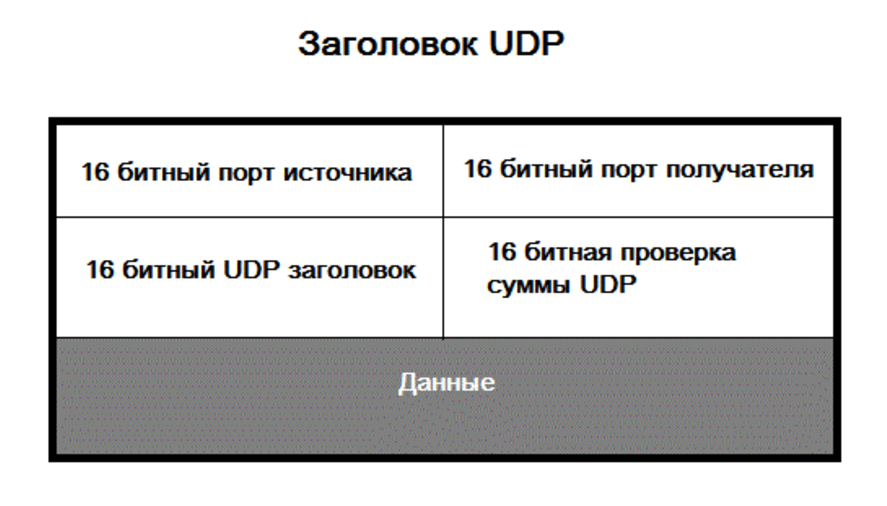
\includegraphics[width=0.9\textwidth]{pics/udp-segment.png}
  \caption{Структура UDP-заголовка}
  \label{udp-header}
\end{figure}

Из полезной информации можно выделить только номера портов и поле <<Данные>>.

Стоит отметить, что RDP использует UDP в случаях, когда нужно минимизировать задержки и повысить производительность, особенно для мультимедийных 
задач или нестабильных сетевых условий \cite{udpseg}. Однако TCP остаётся основным протоколом для критически важных операций, таких как 
управление соединением и передача данных с высокой надежностью.

% Далее необходимо рассмотреть методы обнаружения RDP-трафика, которые позволят эффективно выявить наличие использования RDP-протокола.

Рассмотрение структуры пакетов, представленной в данном разделе, позволяет получить общее представление о принципах организации передачи данных в сетях и месте 
протокола RDP в стеке сетевых протоколов. Однако для решения задачи идентификации RDP-трафика среди общего потока данных возникают некоторые сложности.

Во-первых, RDP-трафик обычно передаётся в зашифрованном виде. Даже если программно получить доступе к полю данных в заголовках TCP и UDP, то расшифровка 
содержимого без наличия ключа шифрования становится практически невозможной. Это делает анализ RDP-заголовков недостаточно эффективным для точного 
определения наличия RDP-трафика.

Во-вторых, использование портов для идентификации RDP также не является надёжным методом. Злоумышленники могут изменить стандартный порт, 
применяемый для RDP-соединений, с целью избежать обнаружения. Более того, если на одном устройстве функционирует несколько RDP-сессий, для каждой 
из них могут использоваться разные порты, что дополнительно усложняет задачу анализа.

Таким образом, возникает вопрос: каким образом можно надёжно отличить трафик протокола удалённого рабочего стола от других протоколов, наблюдаемых в сетевой среде?

Ответ на данный вопрос будет рассмотрен в следующем разделе, где проанализированы ключевые метрики и особенности, характерные для RDP-трафика.

\section{Особенности и характерные признаки RDP-трафика}

В рамках моей предыдущей курсовой работы, посвящённой теме <<Статистический анализ сетевого трафика для обнаружения активной RDP-сессии>>, 
были изучены и применены различные методы статистического анализа для выявления RDP-трафика. В частности, рассматривались такие подходы, как:  

\begin{itemize}
  \item анализ распределения временных интервалов между пакетами;  
  \item исследование распределения размера пакетов;  
  \item анализ частоты флагов PSH;  
  \item нахождение отношения входящего и исходящего трафика.  
\end{itemize}

Результаты курсовой работы показали, что использование этих методов в совокупности позволяет с высокой степенью вероятности идентифицировать 
RDP-трафик в сетевой среде.  


В рамках настоящего исследования статистические методы рассматриваются более детально. Они дополняются новыми метриками, 
учитывающими динамические особенности RDP-сессий. Эти признаки используются в качестве входных данных для обучения нейронной сети, что позволяет 
значительно повысить точность и надёжность обнаружения RDP.

В данном разделе подробно описываются признаки, характерные для RDP-трафика и способы расчета метрик на основе этих признаков.
Все представленные метрики сопровождаются формулами и пояснениями их реализации в программной системе. Стоит отметить, что вся информация, 
используемая при вычислении метрик, собирается самой программой. Программа извлекает из перехваченных пакетов исключительно те данные, которые 
требуются для расчёта метрик.

\subsection{Признаки на основе анализа временных интервалов между пакетами}

Анализ временных интервалов между пакетами может помочь выявить RDP-сессии. Как правило, промежутки между пакетами RDP-трафика короче, 
чем у других видов трафика. Это объясняется тем, что протокол RDP рассчитан на передачу данных в реальном времени и требует быстрой 
доставки информации для поддержания стабильного соединения с удаленным рабочим столом. Соответственно, если в сети наблюдается 
большое количество пакетов с короткими временными интервалами, это может свидетельствовать о наличии активной RDP-сессии. Тем 
не менее, важно помнить, что существуют и другие виды трафика, использующие высокие скорости передачи данных и характеризующиеся 
малыми интервалами между пакетами. Поэтому вычисляется несколько метрик, получаемые из промежутков временных интервалов, чтобы улучшить
процесс определения RDP-трафика.

\subsubsection{Вычисление задержки и стандартного отклонения временных интервалов между пакетами}

Под задержкой будем понимать среднее время, которое проходит между отправкой и получением пакетов. Пусть $ t_1, t_2, \dots, t_n $, 
где $ t_i $ --- это временная метка $ i $-го пакета. Разработанная программа запоминает все эти временные метки и находит разницу ($\Delta t_j$) 
между двумя пакетами следующим образом:
\begin{equation}
  \Delta t_j = t_{i+1} - t_{i}, \text{ для всех } i = \overline{1, n - 1}
\end{equation}

Тогда задержка вычисляется по следующей формуле:

\begin{equation}
  \mu_L = \frac{1}{n - 1} \sum_{i=1}^{n-1} \Delta t_i
\end{equation}

Исходя и формулы (2) можно заметить, что задержка --- это среднее значение временных интервалов между пакетами.

Вычисление стандартного отклонения, получается из значения задержки по следующей формуле:

\begin{equation}
  \sigma = \sqrt{\frac{1}{n-1} \sum_{i=1}^{n-1} (\Delta t_i - \mu_L)^2}
\end{equation}

  Среднее значение (задержка) и стандартное отклонение позволяет оценить стабильность интервалов времени 
  и, следовательно, стабильность передачи данных, что является одной из характерных черт RDP-трафика.

\subsubsection{Вычисление среднего джиттера и медианы временных интервалов}

   Джиттером называется изменение временной задержки между передачей данных и их получением по сетевому соединению.
   Проще говоря, джиттер отражает нестабильность задержки. Данная величина вычисляется по следующей формуле:

   \begin{equation}
      J_i = |\Delta t_{i+1} - \Delta t_i|, \quad \text{для } i = \overline{1, n - 2}.
   \end{equation}

  Тогда средний джиттер вычисляется следующим образом:

   \begin{equation}
    \mu_J = \frac{1}{n-2} \sum_{i=1}^{n-2} J_i
   \end{equation}

   Этот показатель характеризует, насколько стабильны интервалы между пакетов, что важно для оценки качества RDP-сессий, 
   поскольку низкий джиттер необходим для стабильной работы удаленного рабочего стола. 
   
   Исходя из формул вычисления задержки и джиттера может показаться, что эти величины похожи, но это не так. Они измеряют разные 
   аспекты передачи данных, и каждая из этих метрик имеет свое значение в контексте анализа RDP-трафика. Задержка показывает, как долго 
   передаются пакеты, а джиттер измеряет колебания этого времени.

   Медиана временных интервалов является также полезной метрикой, которая может помочь сгладить влияние выбросов и экстремальных значений. 
   Медиана представляет собой среднее значение в отсортированном ряду интервалов времени. Вследствие этого временные метки $t_i$ ($i = \overline{1, n}$) 
   перехваченных пакетов сортируются по возрастанию.
   
   Далее если количество интервалов $ n $ нечетное, то медианой будет центральный элемент отсортированного ряда. 
   Если $ n $ четное, медианой будет среднее значение двух центральных элементов.

   Таким образом медиана вычисляется следующим образом:

   \begin{equation}
    m_t = 
      \begin{cases}
        t_{n / 2}, & \text{если n нечетное}\\
        (t_{n / 2} + t_{n / 2 + 1}) / 2, & \text{если n четное}
      \end{cases}
   \end{equation}
  

\subsection{Признаки, связанные с количественными характеристиками трафика}


Помимо анализа временных интервалов, важную информацию о характере трафика можно получить из количественных характеристик передаваемых пакетов.
Анализ объёма и распределения трафика позволяет выявить ключевые закономерности, присущие протоколу RDP. Такие признаки, как соотношение 
входящего и исходящего трафика, распределение объёмов между UDP- и TCP-пакетами, а также средний размер передаваемых пакетов, отражают 
особенности поведения RDP-сессий. Каждый сетевой протокол обладает уникальным паттерном обмена данными, и изучение этих характеристик 
играет важную роль в их идентификации.

\subsubsection{Вычисление отношения объема входящего на исходящий трафик}

Разработанная программа сохраняет пакеты относительно инициатора подключения (клиента) и целевого устройства (сервера). В процессе работы накапливаются 
две величины: объем исходящего трафика ($V_{src}$) — количество данных, отправляемых клиентом, и объем входящего трафика ($V_{dest}$) — количество данных, 
отправляемых сервером.

Отношение объема входящего на исходящий трафик вычисляется по формуле:

\begin{equation}
  r_{dest/src}^{init} = \frac{V_{dest}}{V_{src}}
\end{equation}

Аналогично отношение объема трафика относительно сервера вычисляется как:

\begin{equation}
  r_{dest/src}^{targ} = \frac{V_{src}}{V_{dest}}
\end{equation}

Эти две величины позволяют оценить симметричность обмена данными между клиентом и сервером. Для протокола RDP характерен асимметричный обмен 
трафиком: большая часть данных передается от сервера к клиенту, что обусловлено характером работы протокола, где сервер передает графическую 
информацию, а клиент отправляет команды управления.

Рассмотрение обеих величин важно, поскольку оно обеспечивает всесторонний анализ взаимодействия между клиентом и сервером. Например, высокое 
значение $r_{dest/src}^{init}$ (преобладание входящего трафика) может указывать на активность RDP-сессии, тогда как отклонения в этих показателях 
могут сигнализировать о другом типе соединения. Метрика особенно полезна в контексте других признаков, так как её устойчивость к шуму и вариативность 
в зависимости от типа трафика делает её важным элементом для классификации с использованием нейронной сети.

\subsubsection{Вычисление отношения объема UDP-трафика и TCP-трафика}

В предыдущем разделе упоминалось, что начиная с версии 8.0, протокол RDP поддерживает передачу данных по UDP. Это особенно заметно в 
сетевом обмене между компьютерами с установленной операционной системой Windows. По протоколу UDP в основном передаются графические данные, 
а также действия, совершаемые мышью и клавиатурой, что делает его важной частью работы RDP. Учитывая это, исключать анализ UDP-трафика из 
общей картины трафика было бы неправильно.

Разработанная программа отслеживает объем переданных пакетов по протоколам UDP и TCP, а также вычисляет их соотношение по следующей формуле:

\begin{equation}
  r_{udp/tcp} = \frac{V_{udp}}{V_{tcp}}
\end{equation}

Таким образом, данная метрика отражает баланс использования двух транспортных протоколов в рамках одного соединения. Для RDP характерно 
заметное преобладание трафика по протоколу TCP, однако наличие UDP-трафика с характерным объемом может служить дополнительным индикатором 
активности RDP-сессии.

Эта метрика становится особенно эффективной в сочетании с другими признаками, улучшая точность классификации сетевого трафика и выявления RDP.

\subsubsection{Вычисление среднего значения объема пакетов}

При работе протоколов прикладного уровня данные передаются пакетами различных объемов. 
Размер пакетов может варьироваться в зависимости от характера передаваемой информации: от небольших управляющих сообщений до крупных сегментов данных
Исследование размеров передаваемых пакетов может оказаться полезным инструментом при анализе сетевого 
трафика, особенно когда речь идет об определении аномалий или подозрительных активностей.


В разработанной программе анализируется размер блока «Данные», содержащегося в заголовках протоколов TCP и UDP. В процессе перехвата 
трафика программа сохраняет размеры полезной нагрузки каждого пакета: $p_{s_1}, p_{s_2}, \dots, p_{s_n}$. На основании этих данных 
вычисляется среднее значение объема передаваемых пакетов:

\begin{equation}
  \mu_P = \frac{1}{n} \sum_{i=1}^{n} \Delta p_{s_i}
\end{equation}

Эта метрика предоставляет информацию о характере передаваемого трафика. Для протокола RDP характерен обмен пакетами малого и среднего 
размера, отражающий отправку управляющих сигналов, таких как движения мыши, нажатия клавиш, или обновления небольших частей экрана. В 
отличие от этого, потоки мультимедиа или файлы, передаваемые другими протоколами, обычно характеризуются значительно большими средними 
размерами пакетов.

Значимость среднего значения объема пакетов заключается в его способности идентифицировать типичные характеристики RDP-сессий и исключать 
несоответствующий трафик, тем самым улучшая точность анализа и классификации. В сочетании с другими метриками эта характеристика позволяет 
более точно выделять RDP-трафик среди общего потока сетевых данных.

\subsection{Признаки на основе анализа параметров TCP-соединений}

Протокол TCP предоставляет множество полей в своих заголовках, каждое из которых несет важную информацию о состоянии соединения, обмене данными и 
управлении потоком. Эти параметры играют ключевую роль в обеспечении надёжности передачи данных, но также могут служить источником ценной информации 
для анализа сетевого трафика.

В результате детального изучения особенностей сетевого взаимодействия по протоколу RDP были выявлены признаки, которые позволяют отличить данный 
тип трафика от других. Эти признаки связаны с использованием управляющих флагов TCP (PSH, ACK, SYN, FIN, RST), размером окна и другими параметрами, 
которые характеризуют поведение соединения.


\subsubsection{Вычисление частоты флагов PSH и ACK}

В контексте протокола RDP флаг PSH активно применяется для передачи пользовательских действий, таких как нажатия клавиш и движение мыши, 
а также для пересылки буферизованных изображений или звуковых данных. Наличие PSH-флагов может быть индикатором активности RDP-сессий, 
что делает их анализ полезным инструментом для идентификации такого трафика.

% Разработанная программа считает количество TCP-пакетов, у которых флаг PSH равен единице, причем она вычисляет относительно клиента и сервера.
% Другими словами, программа считает количество TCP-пакетов с установленным флагом PSH, где клиент выступает в роли получателя. Аналогично считает 
% количество TCP-пакетов с установленным флагом PSH, где сервер выступает в роли получателя. Аналогично считается количество TCP-пакетов, получаемых клиентом и сервером.

% В результате к некоторому моменту времени
% программа получает $V_{P_{src}}$ --- объем входящего трафика с установленным флагом PSH относительно клиента и $V_{P_{dest}}$ относительно сервера, а также 
% $V_{tcp}^{src}$ --- общее число входящих TCP-пакетов получаемых клиентом, $V_{tcp}^{dest}$ --- общее число входящих TCP-пакетов получаемых клиентом. 

Для анализа частоты PSH-флагов разработанная программа подсчитывает количество TCP-пакетов с установленным флагом PSH для каждой стороны соединения. 
Это позволяет выделить:

\begin{itemize}
  \item $V_{P_{src}}$: объем входящего трафика с установленным флагом PSH относительно клиента;
  \item $V_{P_{dest}}$: объем входящего трафика с установленным флагом PSH относительно сервера;
  \item $V_{tcp}^{src}$: общее количество входящих TCP-пакетов, получаемых клиентом;
  \item $V_{tcp}^{dest}$: общее количество входящих TCP-пакетов, получаемых сервером.
\end{itemize}

На основе этих данных вычисляются частоты флагов PSH для каждой стороны.

Для клиента:

\begin{equation}
  r_{psh}^{init} = \frac{V_{P_{src}}}{V_{tcp}^{src}}
\end{equation}

Для сервера:

\begin{equation}
  r_{psh}^{targ} = \frac{V_{P_{dest}}}{V_{tcp}^{dest}}
\end{equation}

Анализ частоты PSH-флагов позволяет выявить характерный для RDP трафик, где их интенсивность выше, чем у большинства других протоколов. 
Рассмотрение этих метрик как относительно клиента, так и относительно сервера важно для учёта специфики взаимодействия между сторонами: 
данные клиента часто включают команды, а данные сервера — графическую или звуковую информацию. Такой двусторонний анализ помогает точнее 
охарактеризовать тип и особенности обмена данными.

\subsubsection{Вычисление отношения ACK/PSH}
\subsubsection{Вычисление разности числа исходящих и входящих ACK-флагов}


\subsubsection{Вычисление отношения количества флагов SYN на сумму флагов FIN + RST}
\subsubsection{Вычисление среднего значения размера окна}



\subsection{Анализ признаков RDP-трафика относительно других протоколов}

\subsection{Метрики, используемые для классификации}


\conclusion
  
Заключение

  \begin{thebibliography}{15}
    \bibitem{lib1}
    Фаткиева, Р. Р Разработка метрик для обнаружения атак на основе анализа сетевого трафика / Р. Р. Фаткиева // Вестник Бурятского государственного университета, выпуск 9, 2013. С. 81-86.
    \bibitem{lib2}
    Карачанская, Е.В Метод выявления аномалий сетевого трафика, основанный на его самоподобной структуре / Е.В. Карачанская, Н.И. Соседова // Безопасность информационных технологий, том 26, №1, 2019. С. 98-110.
    \bibitem{2}
    Alexey Удалённый рабочий стол RDP: как включить и как подключиться по RDP [Электронный ресурс] : настройка удаленного рабочего стола RDP. -- URL: https://hackware.ru/?p=11835\#11 (дата обращения: 31.03.2023). -- Загл. с экрана. -- Яз. рус.
    \bibitem{rdp2}
    https://learn.microsoft.com/en-us/troubleshoot/windows-server/remote/understanding-remote-desktop-protocol
    \bibitem{stack}
    https://cyberleninka.ru/article/n/semiurovnevaya-model-osi-iso-i-stek-protokolov-tcp-ip-issledovanie-vzaimootnosheniya-i-interpretatsii/viewer
    % \bibitem{rdp2}
    % Remote Utilities RDP [Электронный ресурс] : подключение к удаленному рабочему столу. --  Remote Utilities Pty (Cy) Ltd 2010 -- 2023. -- URL:  https://www.remoteutilities.com/support/docs/rdp/ (дата обращения: 31.03.2023). -- Загл. с экрана. -- Яз. англ.
    \bibitem{osi-model}
    Maintenance script Модель OSI [Электронный ресурс] : описание модели OSI. -- Университет ИТМО. -- URL: http://neerc.ifmo.ru/wiki/index.php?title=OSI_Model (дата обращения: 31.03.2023). -- Загл. с экрана. --  Яз. рус.
    \bibitem{winsize}
    https://learn.microsoft.com/ru-ru/troubleshoot/windows-server/networking/description-tcp-features
    \bibitem{tcpflags}
    KeyCDN TCP flags [Электронный ресурс] : описание TCP-флагов. -- proinity LLC 2023. -- URL: https://www.keycdn.com/support/tcp-flags\#:$\sim$:text=ACK (дата обращения: 31.03.2023). -- Загл. с экрана. --  Яз. англ.
    \bibitem{udpseg}
    https://learn.microsoft.com/en-us/openspecs/windows_protocols/ms-rdpeudp/2744a3ee-04fb-407b-a9e3-b3b2ded422b1
    % \bibitem{socket1}
    % The Python Standard Library Socket - Low-level networking interface [Электронный ресурс] : описание методов библиотеки socket. -- Python Software Foundation 2001 -- 2023. -- URL: https://docs.python.org/3/library/socket.html (дата обращения: 31.03.2023). -- Загл. с экрана. -- Яз. англ.
    % \bibitem{session}
    % How Terminal Services Works [Электронный ресурс] : описание службы терминалов удаленного рабочего стола. -- Microsoft 2023. -- URL:  https://learn.microsoft.com/en-us/previous-versions/windows/it-pro/windows-server-2003/cc755399(v=ws.10)?redirectedfrom=MSDN (дата обращения: 14.04.2023). -- Загл. с экрана. -- Яз. англ.
    % \bibitem{rdp1}
    % Antenore Gatta The fast, stable, and always free Linux RDP client [Электронный ресурс] : подключение по RDP с помощью приложения Remmina. -- URL: https://www.remmina.org/remmina-rdp/ (дата обращения: 15.04.2023). -- Загл. с экрана. -- Яз.  англ.
    % \bibitem{rdpport}
    % Jenks, A. Change the listening port for Remote Desktop on your computer / A. Jenks, S. Manheim, H. Lohr // [Электронный ресурс] : изменение порта прослушивания для RDP. -- Microsoft, 2023. -- URL: https://learn.microsoft.com/ru-ru/windows-server/remote/remote-desktop-services/clients/change-listening-port (дата обращения: 28.04.2023). -- Загл. с экрана. -- Яз. англ.
    % \bibitem{dev0}
    % Киреева, Н. В Исследование трафика локальной сети посредством сетевого анализатора «Wireshark» [Электронный ресурс] : методическая разработка к лабораторной работе / Н. В. Киреева, В.П. Зайкин, Н. Н. Васин // Поволжский государственный университет телекоммуникаций и информатики, Самара, 2010. -- URL: http://ib.psuti.ru/content/metod/методическиеWireshark.pdf (дата обращения 04.05.2023). -- Загл. с экрана. -- Яз. рус.
    % \bibitem{dev1}
    % Standard deviation [Электронный ресурс] : описание нахождения стандартного отклонения. -- Википедия. -- URL: https://en.wikipedia.org/wiki/Standard_deviation (дата обращения 04.05.2023). -- Загл. с экрана. -- Яз. англ.
  \end{thebibliography}

  \appendix

    \section{Код traffic-detection.py}
    % \inputminted[fontsize=\footnotesize, linenos]{Python}{code/traffic-detection.py}


\end{document}